\documentclass{article}

\usepackage{fullpage}
\usepackage{graphicx}
\begin{document}
\title{How to check out assignment repos (and turn them in)}

\maketitle
\section{Forking a repository}
Click on the Fork link in the upper right corner of the repository screen (Fig. 1).  Github will prompt you to decide where the repo should be forked to.  Click on your own username to generate a personal fork of the assignment repository.  This generates a copy of the repository that you can amend as you see fit (for example, adding your responses).  
\begin{figure}[h!]
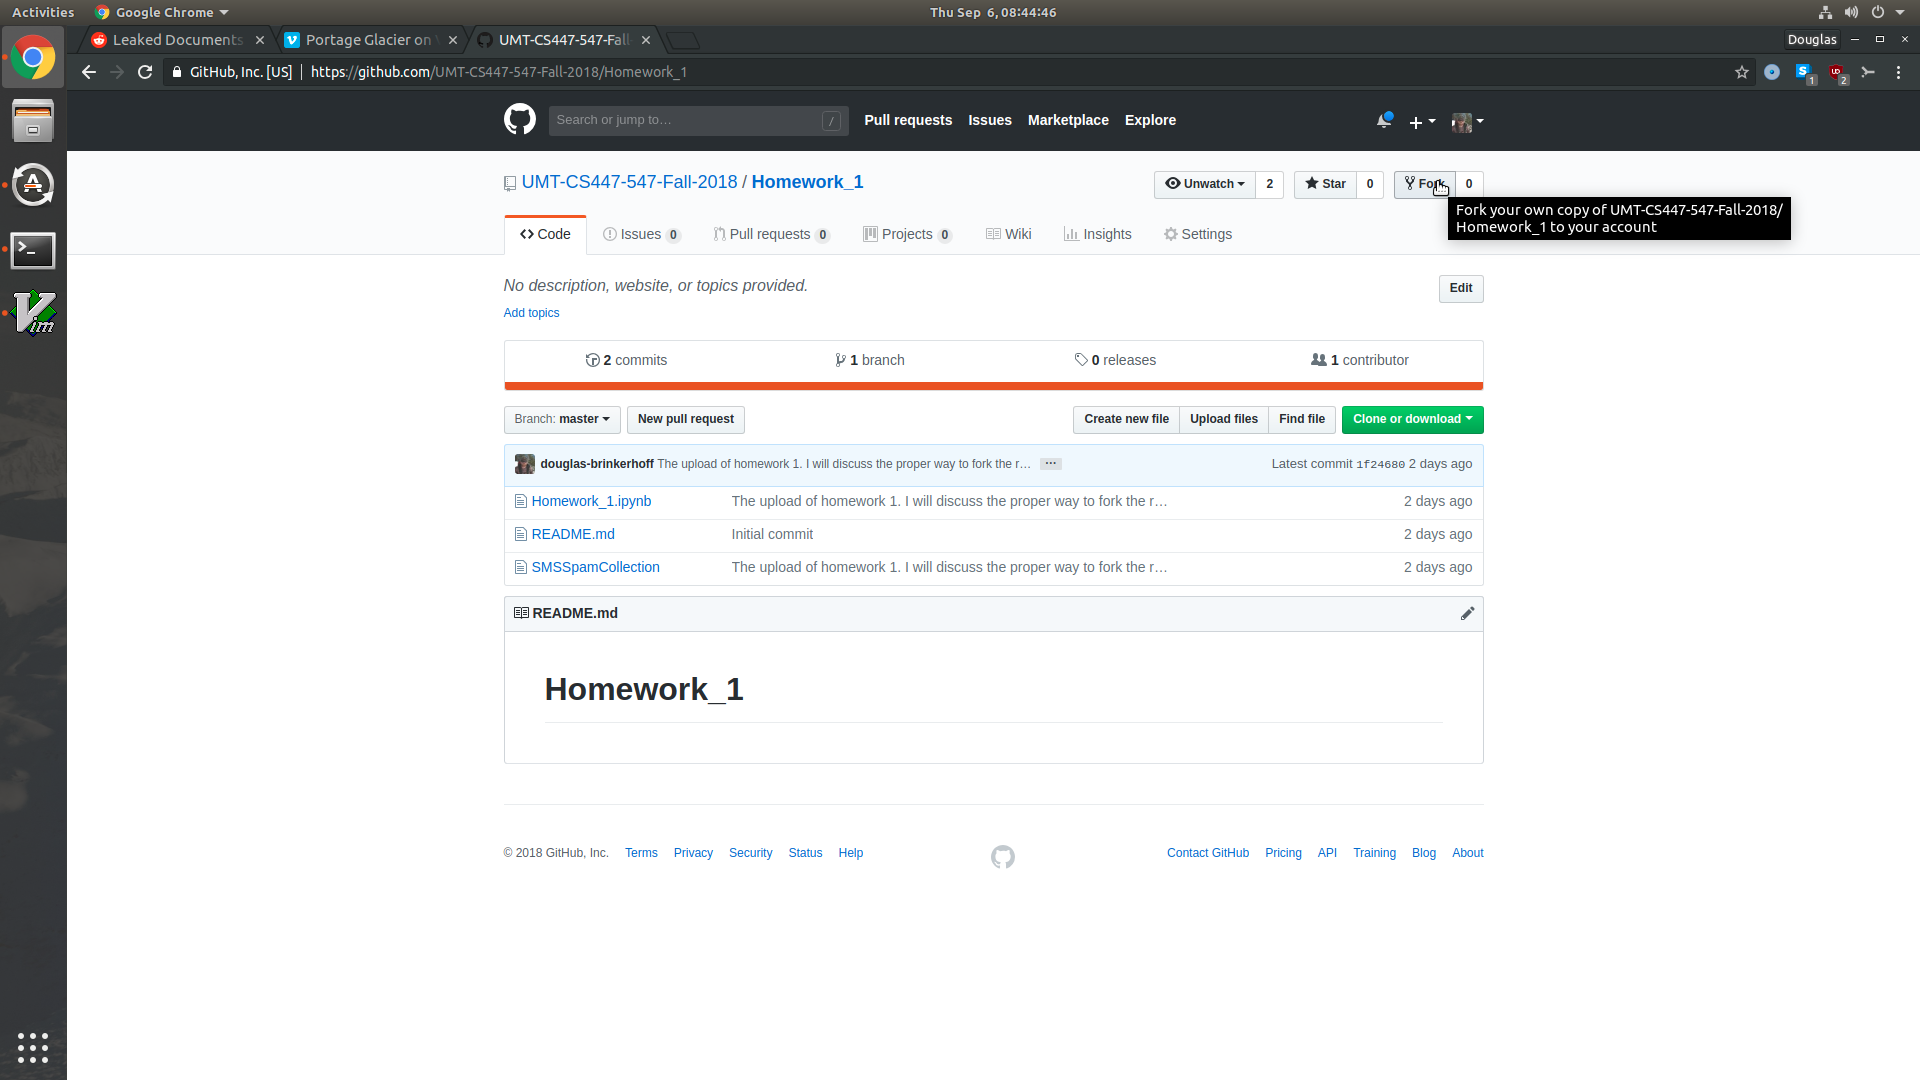
\includegraphics[width=\linewidth]{fork.png}
\caption{Click on this link to fork a repository}
\end{figure}

\newpage

\section{Cloning the repository}
To actually interact with the repository, you'll need to download it to your local machine.  This is called cloning.  To do this, from your personal repository, click the clone or download link (in green) on the right side of the screen (Fig. 2).  This will provide you with a link to the repo.  Copy this link, then open a terminal.  Navigate to wherever you would like your assignment to exist, then type:
\begin{verbatim}
git clone {Link that you just copied}
\end{verbatim}
This will download your fork of the homework repo to your local machine.  
\begin{figure}[h!]
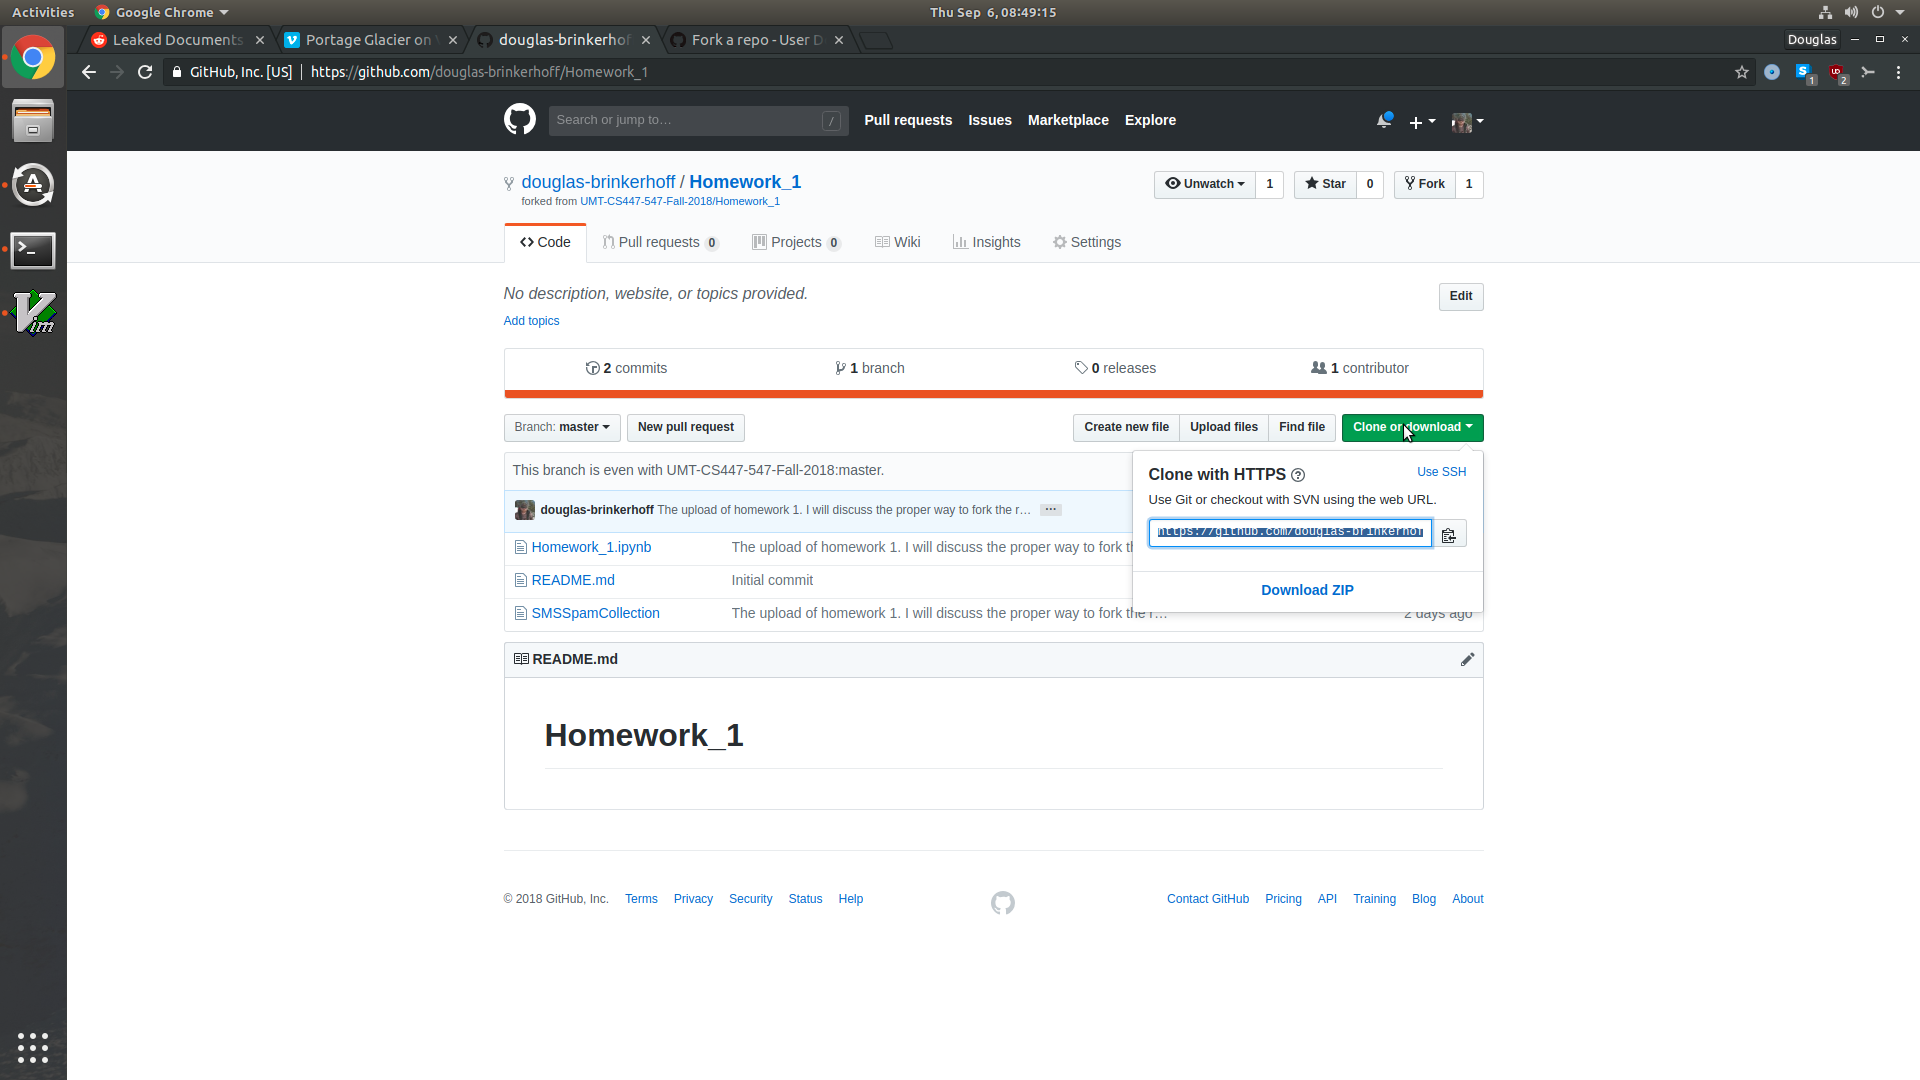
\includegraphics[width=\linewidth]{clone.png}
\caption{Click on this link to fork a repository}
\end{figure}

\newpage


\section{Making edits}
Assignments are distributed as ipython/jupyter notebooks, which means you can use latex markup to write nicely typesetted answers as well as run python code from inside the notebook.  You should provide solutions to the homework problems inside this ipython notebook.  To save your results to git requires two steps.  First, you'll execute the command
\begin{verbatim}
git commit -a -m "A message describing the nature of the changes you made"
\end{verbatim}
This will tell git that you want to save your updated files to the version control system.  Next, to update your personal repository, execute the command
\begin{verbatim}
git push
\end{verbatim}
This will upload the changes you made to your personal fork.  Note that you are not done yet!

\newpage

\section{Turning in your assignment with a pull request}
github supports so-called pull requests, which are requests by a fork (your branch) to be merged into the master branch (my branch).  This is useful because it provides a forum that we can use to discuss the submission, and keeps them all nice and organized in one place for me.  Simultaneously, you maintain your assignments as repositories that you own, which allows you to add them to a coding portfolio, refer to them later, and generally use them how you wish forever.  

To make a pull request, find the \textbf{New pull request} button just above the list of repository files in the main repository (not your fork).  Click this button (Fig. 3).  We're going to be performing a pull request for a fork, so click on the blue text that says compare across forks (Fig. 4).  Under the \textbf{head fork} dropdown menu, locate and select your fork of the repository (Fig. 5).  So long as you've made some changes, you should see a diff of the two repositories, and an option to \textbf{Make pull request} (Fig. 6).  Click this button, and you're done.  Note that you can continue to edit your local fork, and these changes will automatically make it into your pull request (so long as you commit and push these changes as described in the previous section).  
\begin{figure}[h!]
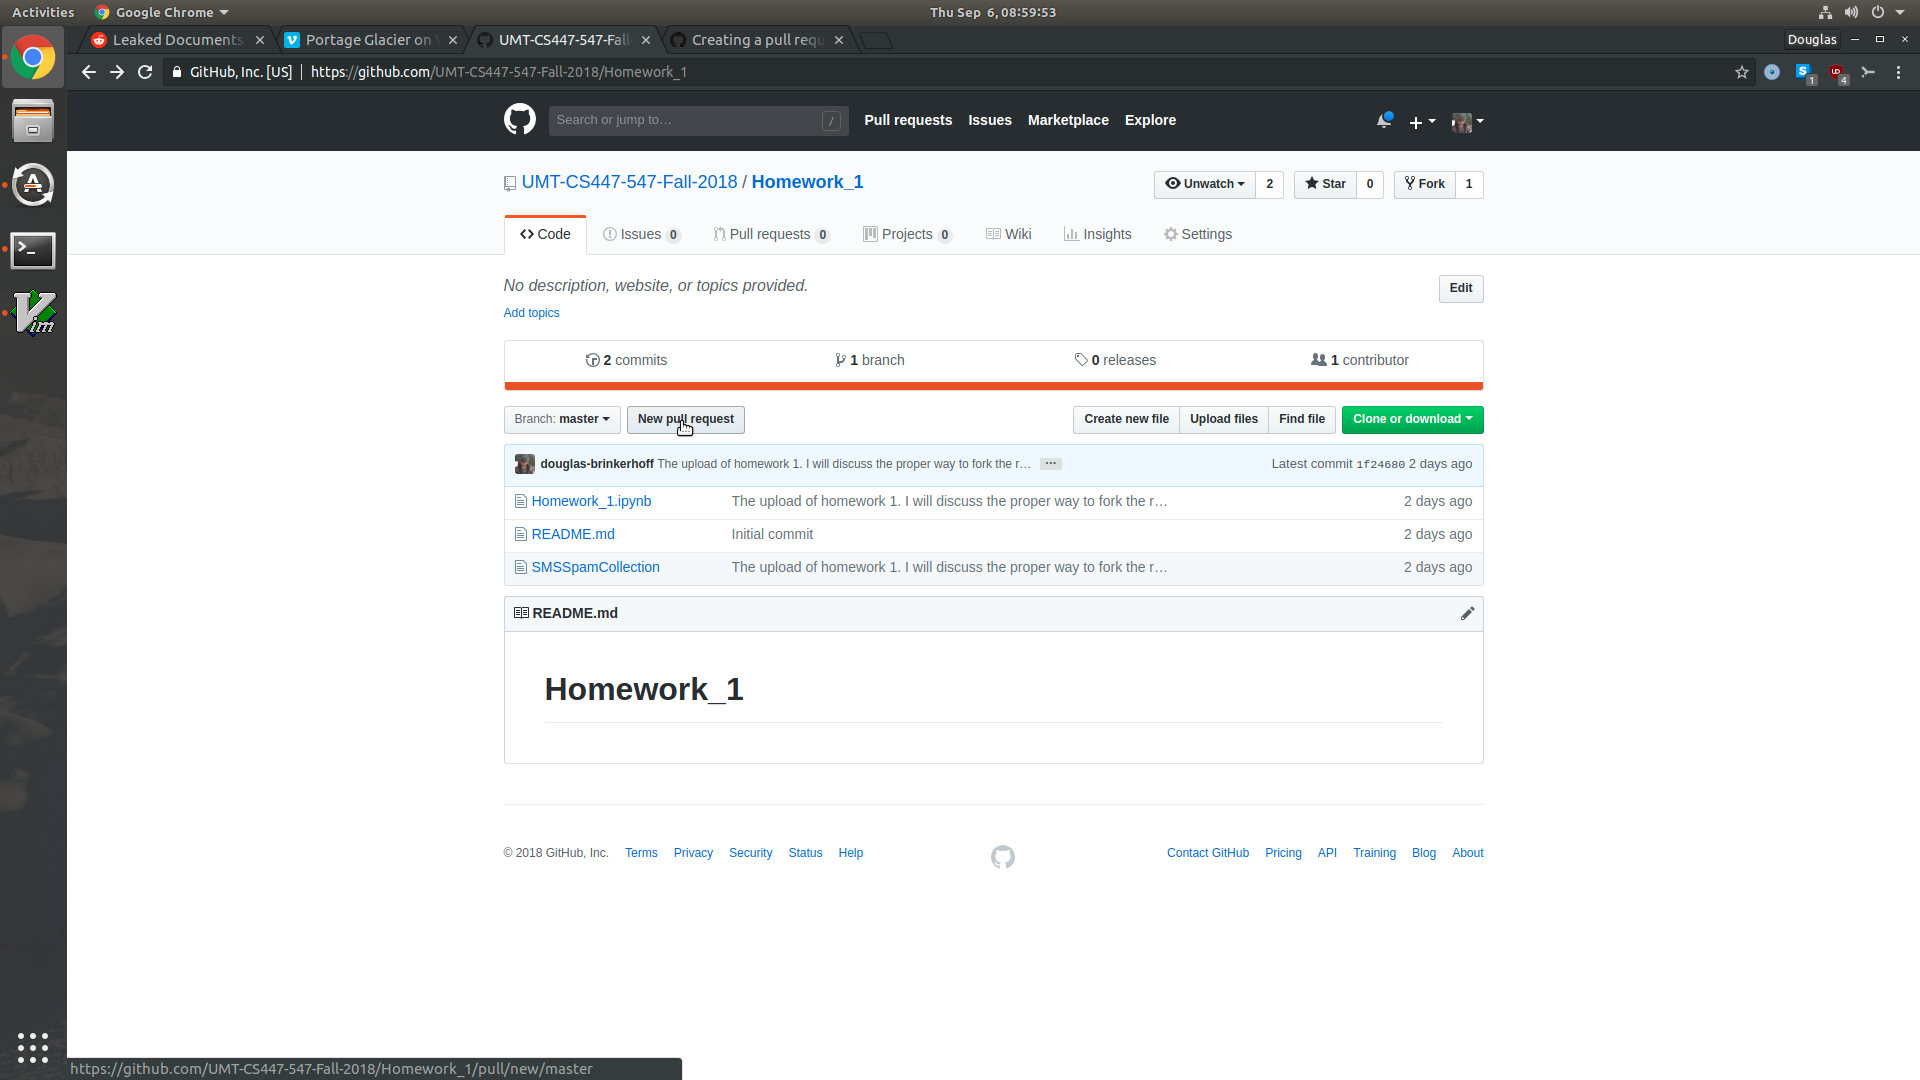
\includegraphics[width=\linewidth]{pull_request_1.png}
\caption{The \textbf{New pull request} button.}
\end{figure}
\begin{figure}[h!]
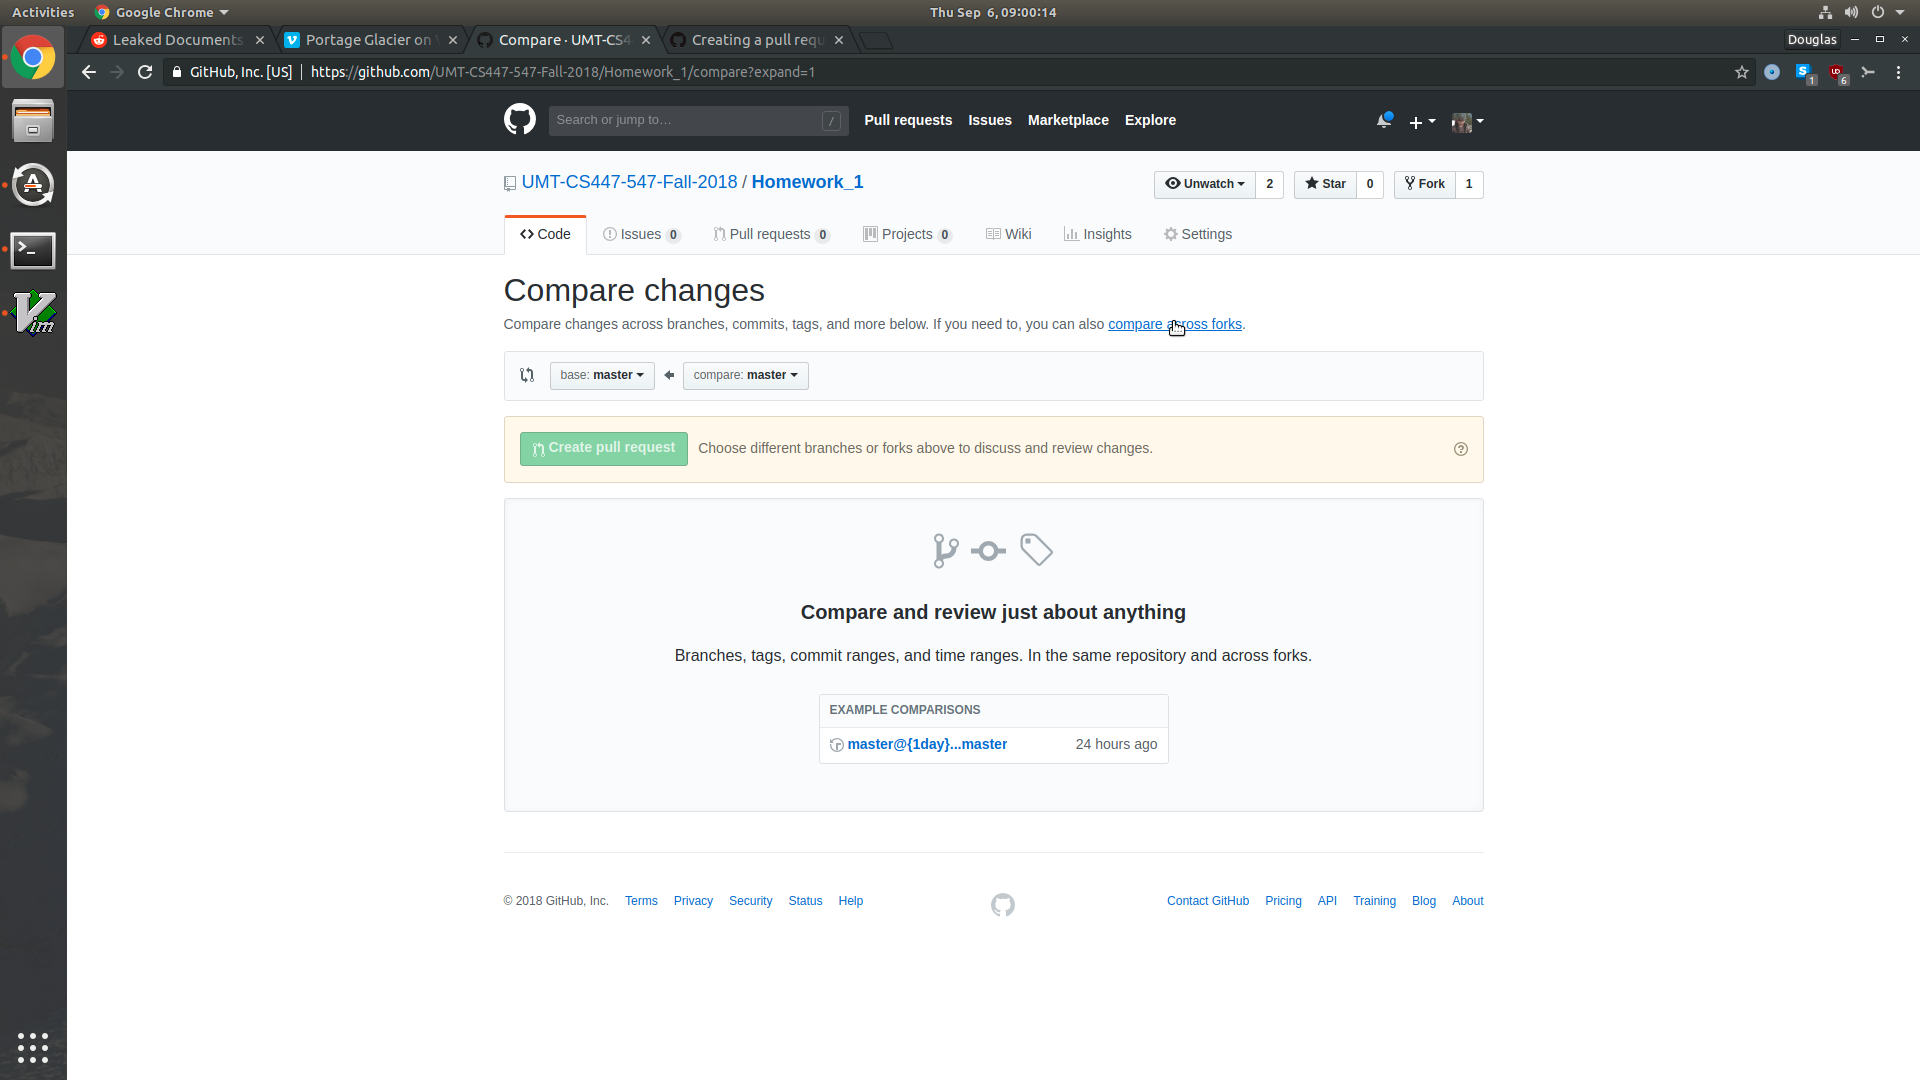
\includegraphics[width=\linewidth]{pull_request_2.png}
\caption{The \textbf{Compare across forks} button.}
\end{figure}
\begin{figure}[h!]
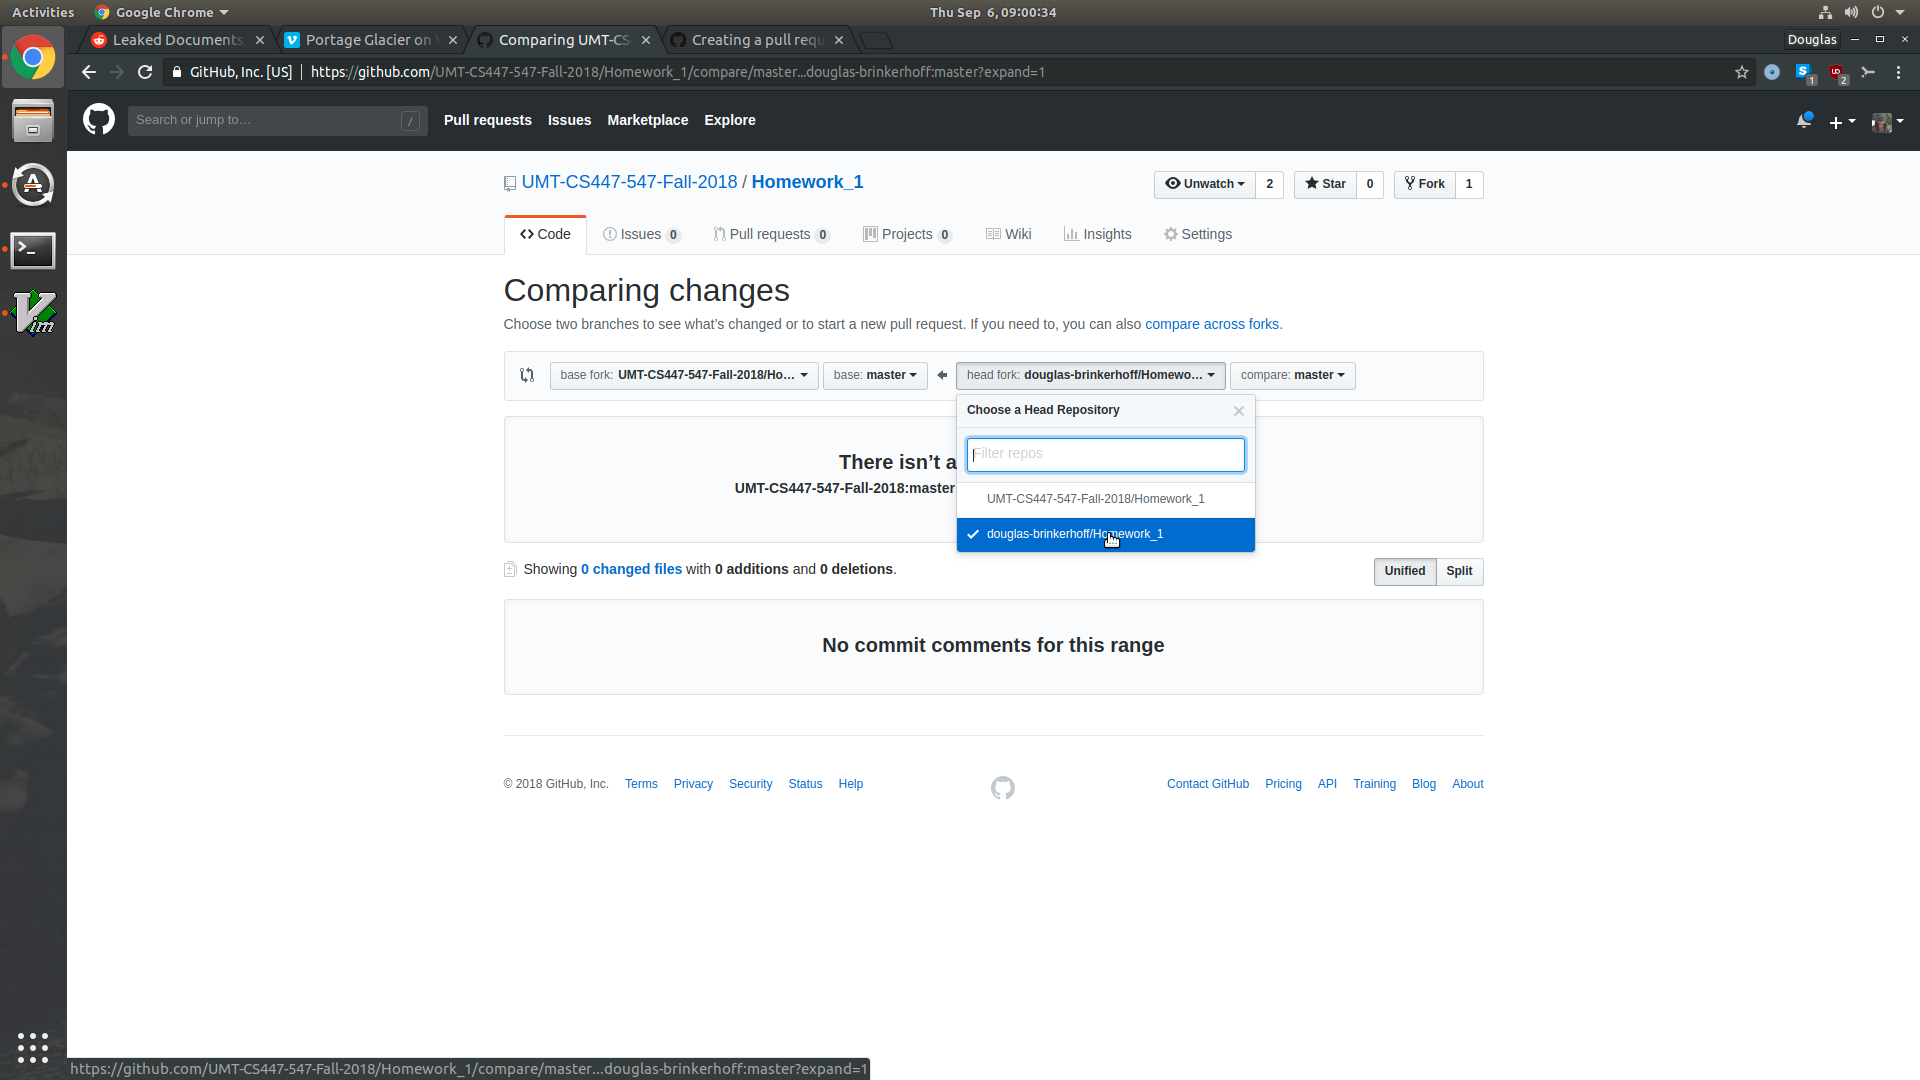
\includegraphics[width=\linewidth]{pull_request_3.png}
\caption{Selecting the repository to add to the pull request.}
\end{figure}
\begin{figure}[h!]
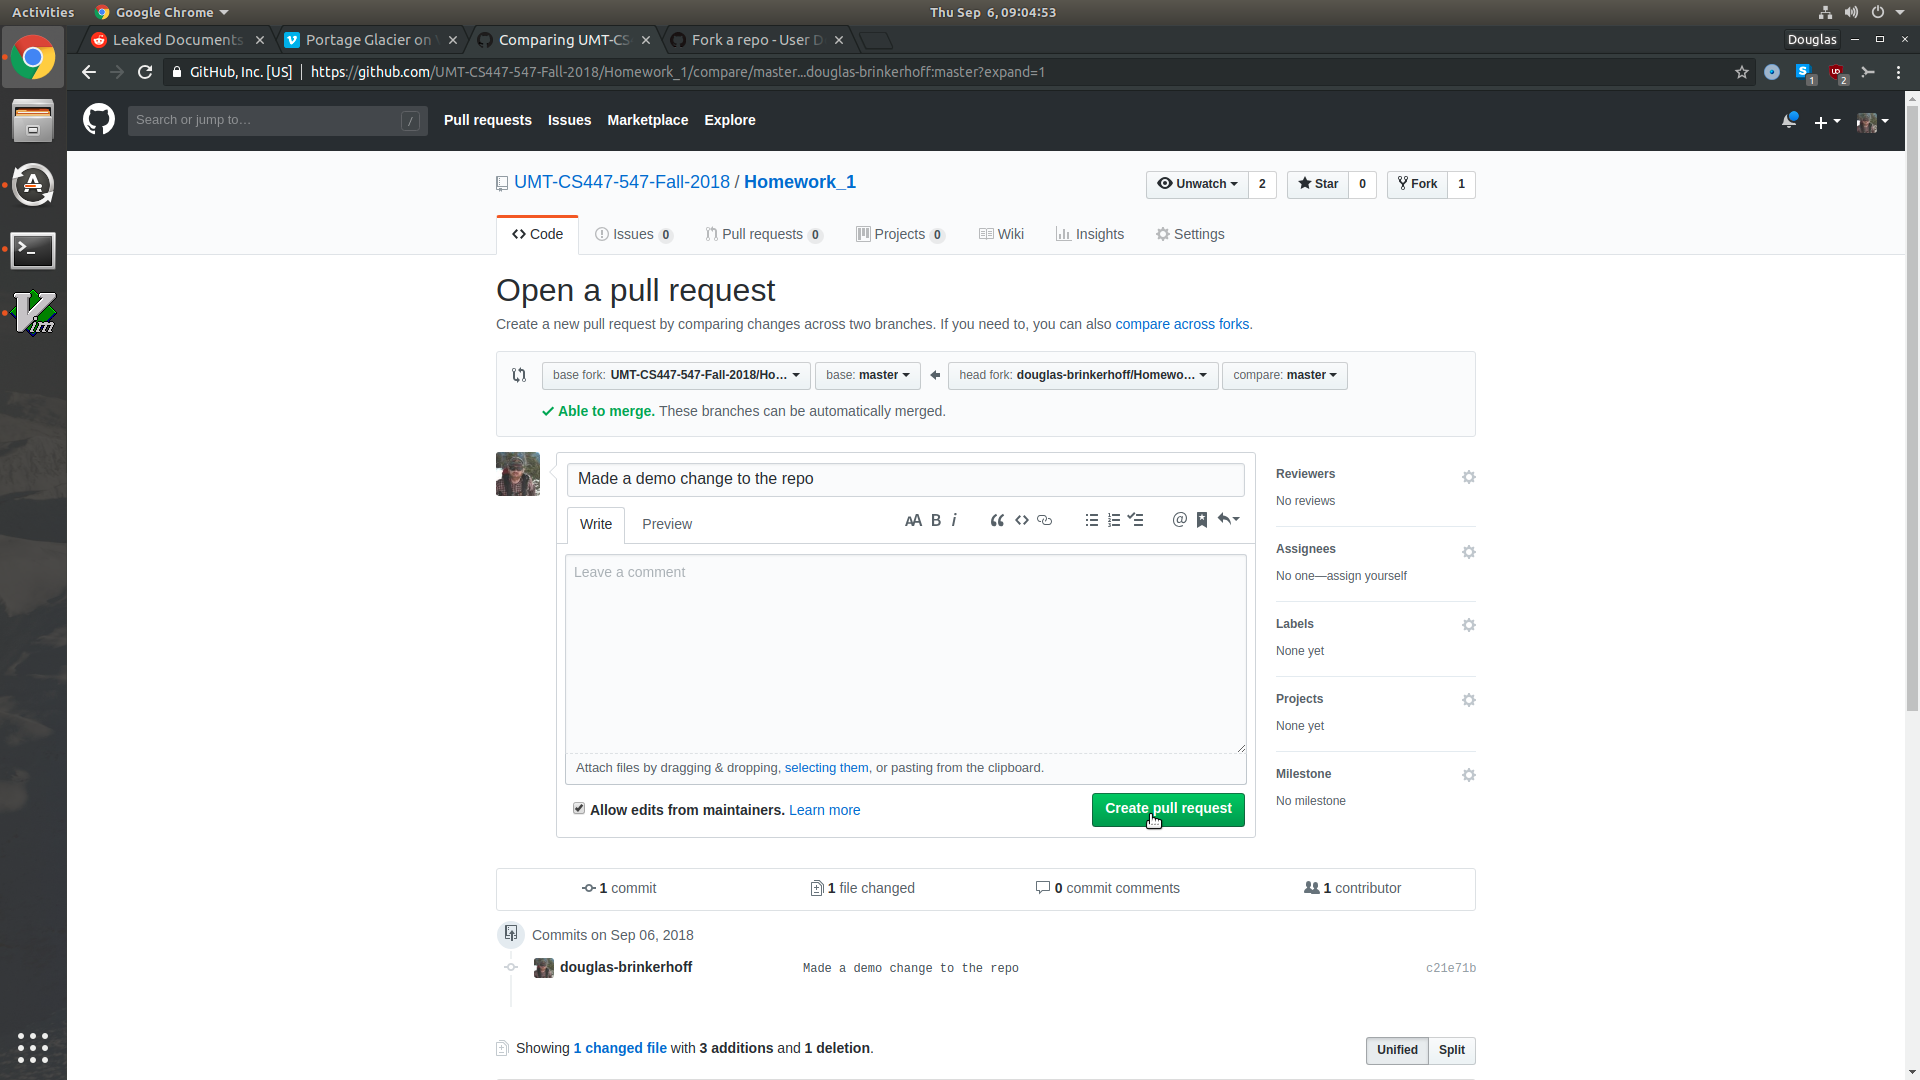
\includegraphics[width=\linewidth]{pull_request_4.png}
\caption{Submitting the pull request.}
\end{figure}

\newpage

\section{Keeping your forked repository synced with the main branch}
Sometimes, I might make changes to the homework assignment after you've forked your branch (typically clarifications and additions.  I'll never do anything that requires you to redo your work).  To keep up to date with these changes, you'll need to set your repository to look for them.  To do this, we'll set an additional \emph{upstream repository}, namely the master branch.  Navigate to your local repository, then use the command
\begin{verbatim}
git remote add upstream {Clone link to master repository}
\end{verbatim}
This tells your local repository to look at the master for possible changes.  Next, you can merge changes in the master into your local branch with the commands
\begin{verbatim}
git fetch upstream
\end{verbatim}
followed by a
\begin{verbatim}
git merge upstream/master
\end{verbatim}
Note that upon execution of this latter command, you may be prompted to include a message by your terminal opening a text editor.  Just save and quit.  Now your local repository (the one on your machine) will be up to date with the master.  Remember that to save these changes to your github repository, you still need to commit and push.

\end{document}








